\begin{frame}{Section 2}
    \begin{itemize}
        \item Get equation $x = y$
        \begin{itemize}
            \item $x \sim$ Uni$(0, 1)$
            \item \textcolor{blue}{To have a blue color $X_0$}
            \item package: tikz 
                \begin{itemize}
                    \item 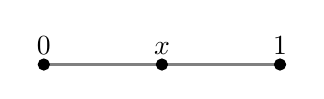
\begin{tikzpicture}
                        \draw[gray, thick] (0, 0) -- (3, 0);
                        \filldraw[black] (0,0) circle (2pt) node[anchor=south]{0};
                        \filldraw[black] (1.5,0) circle (2pt) node[anchor=south]{$x$};
                        \filldraw[black] (3,0) circle (2pt) node[anchor=south]{1};
                    \end{tikzpicture}
                \end{itemize}
        \end{itemize}
    \end{itemize}
\end{frame}


\begin{frame}{Chart}
    \begin{itemize}
        \item To have Objective Function
        \begin{center}
            $\max\limits_{x \geq 0} \ \beta x a^T + (1 - \beta) x a^A$
        \end{center}
        \item To have a Chart
    \end{itemize}
      \\
    \begin{table}[!h]
        \begin{center}
            \begin{tabular}{ c|c|c } 
                    & C & D \\ 
             \hline
             A  & $t_{AC}$   & $t_{AD}$ \\ 
             \hline
             B  & $t_{BC}$   & $t_{BD}$ \\
            \end{tabular}
            \caption*{Table 1}
            % \label{Table 1:}
        \end{center}
    \end{table}
\end{frame}


